\section{The \Next\ apparatus}
\label{sec.next100}

\begin{figure}[htbp!]
\centering
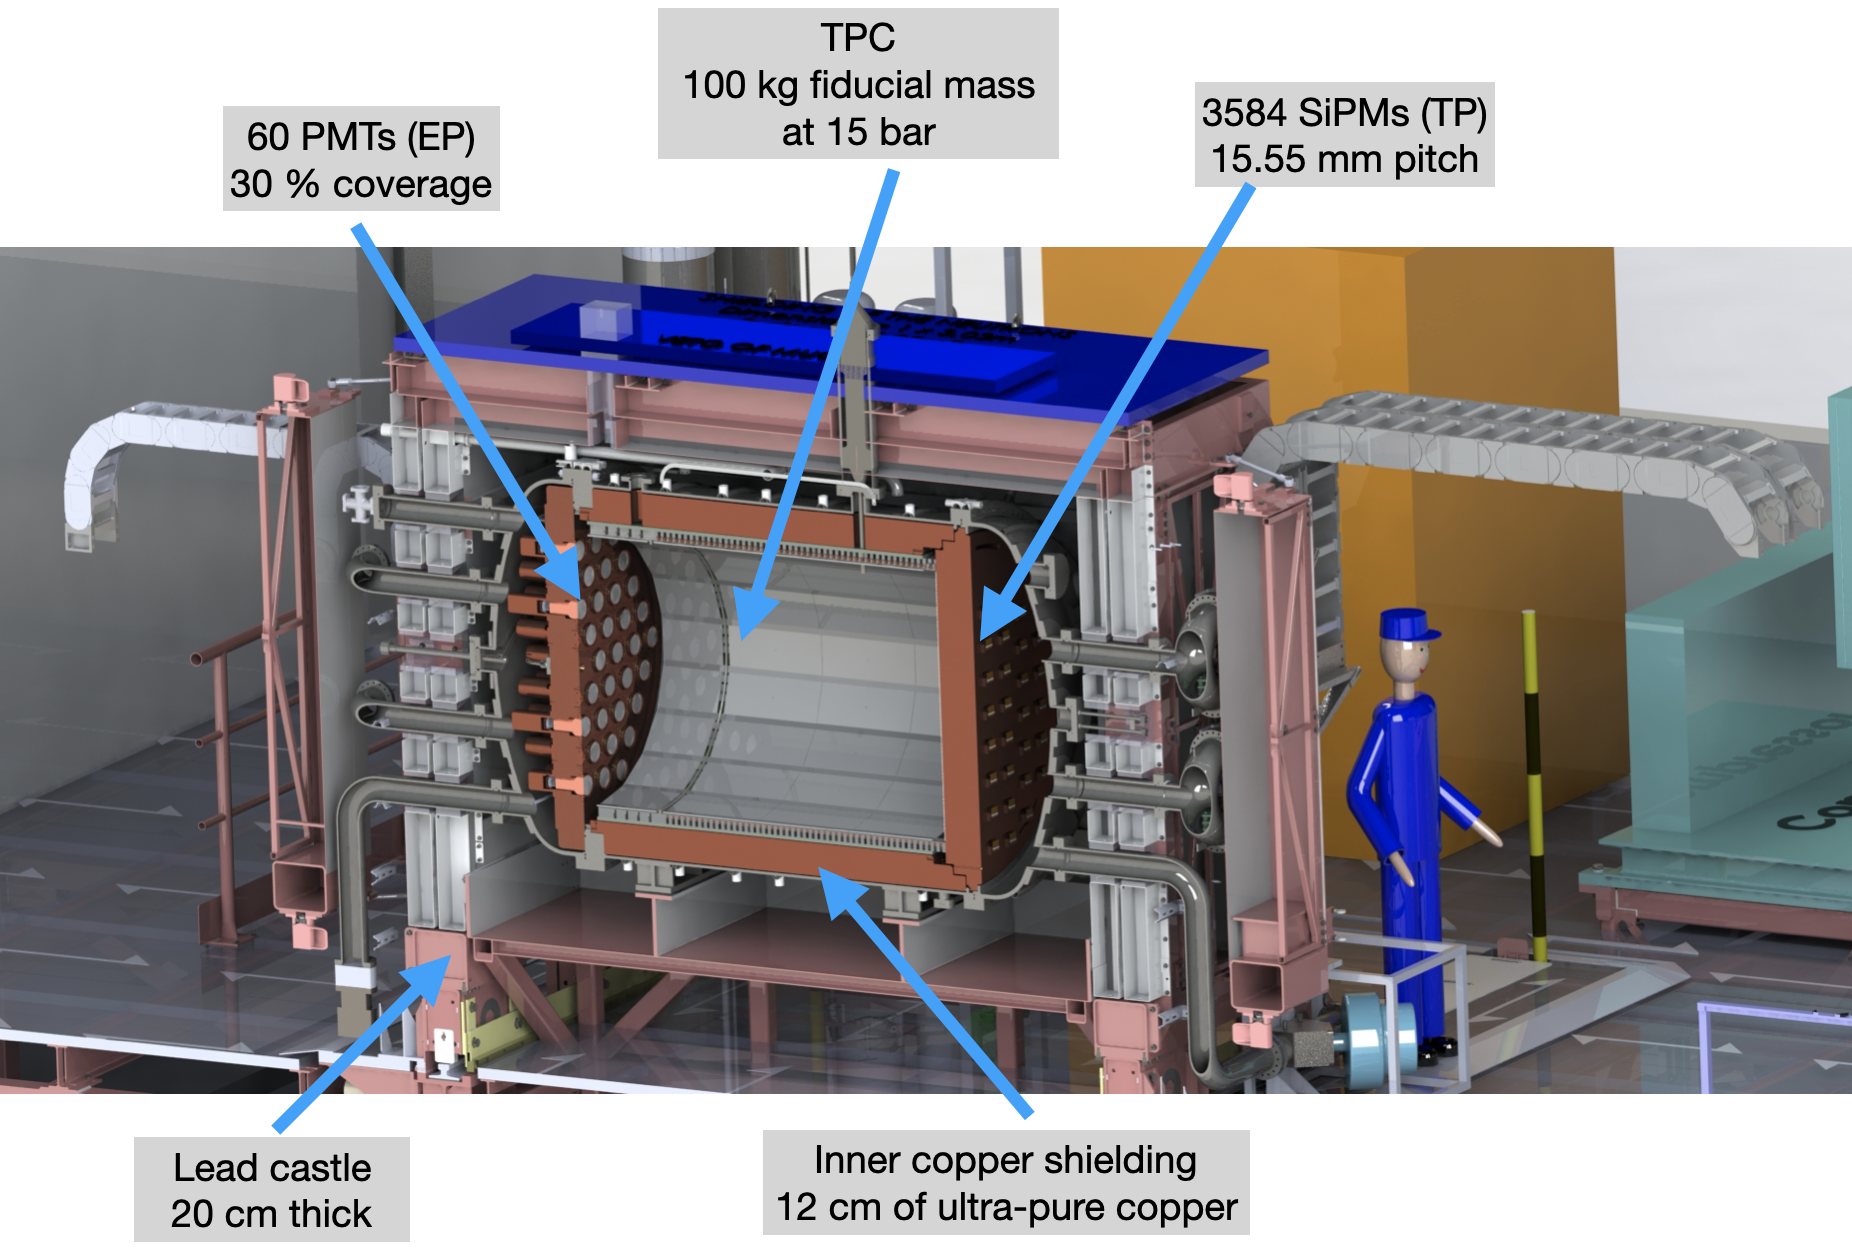
\includegraphics[width=0.9\textwidth]{img/NEXT-100-description.png}
%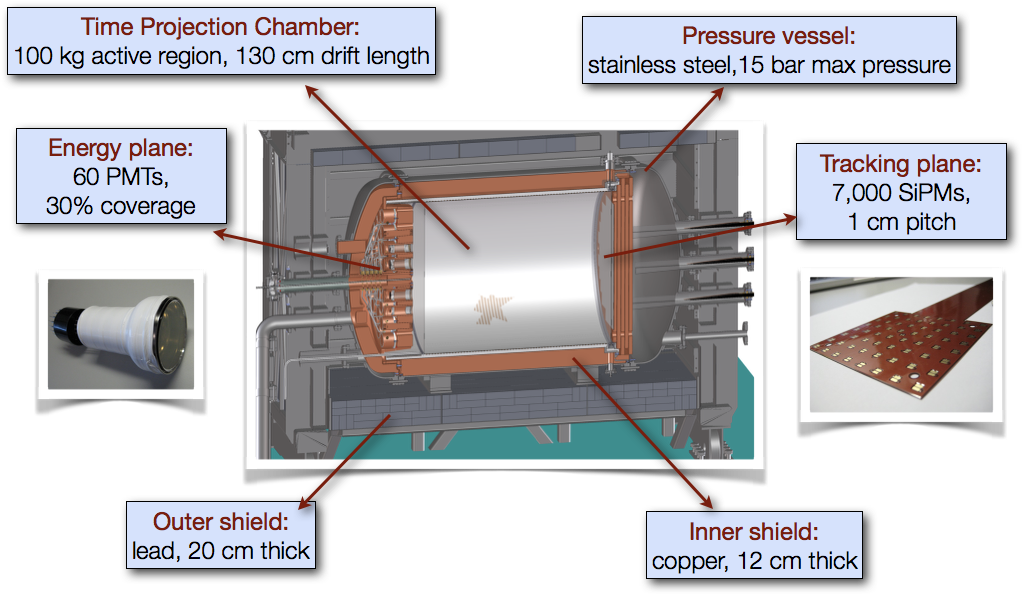
\includegraphics[width=0.9 \textwidth]{img/next-100.png}
\caption{\small Scheme of the \NEXT\ detector.}
\label{fig.next-100}
\end{figure}

\subsection{The detector}
The \Next\ detector is an asymmetric \HPXeEL TPC shown schematically in Figure \ref{fig.next-100}.  The fiducial region is a cylinder of \NextTpcDiameter\ diameter and \NextTpcLength\ length, (\NextFiducialVolume\ fiducial volume) holding a mass of \NextFiducialMass\ of xenon gas enriched at \XeEnrichment\ in \XE, and operating at \NextPressure.  An energy plane (EP),
made of PMTs, provides a measurement of the energy integrating the full signal (\stwo) and records the primary scintillation light (\sone) which triggers the start-of-event (\tz). A tracking plane (TP) provides a 2D image of the tracks propagating in the detector, which is then turned into a 3D image when combined with the measurement of the drift time.  

The TPC consists of a field cage, a cathode held at high voltage via a high-voltage feedthrough, and two electroluminescent meshes for the signal amplification.
The field cage is designed to be a scalable solution for larger system (e.g, for \NHD).  The design is based on affixing copper rings to HDPE staves that run the length of the drift and buffer regions.  
A resistor chain along the field cage copper rings maintains a uniform electric field. Segmented light reflector panels made of Teflon inserted into vented grooves in the HDPE staves provide enhanced light collection, and the full field cage is wrapped in a thin polyethylene insulating sheet to avoid electrical breakdowns between the field cage rings and the outer copper shielding.
The cathode, the anode and the gate (the latter two defining the EL region) consist of three large meshes.  Each mesh will consist of three large parts; the photo-etched mesh that is trapped and tensioned by a two-part frame. This design is the result of a four-year R$\&$D program.

The EP is made of 60 Hamamatsu R11410-10 photomultiplier tubes located behind the TPC cathode, with a coverage of approximately 30\%. This represents a compromise between the need to collect as much light as possible for a robust measurement of the energy and t$_0$ with minimal cost, technical complexity and radioactivity. The R11410-10 is a 3-in PMT especially developed for low-background operation, equipped with a synthetic silica window and a photocathode made of low temperature bialkali with quantum efficiency above 30\% for the emission wavelengths of xenon and TPB.

The R11410-10 cannot be run above 6 atmospheres. To overcome this limitation, the PMTs are housed in a vacuum region behind 5 mm thick sapphire windows (Fig. \ref{fig.EP}). The PMTs are optically coupled to the windows using an optical gel with a refractive index intermediate between those of fused silica and sapphire. TPB is evaporatively coated on the external faces of the windows. 
The PMT cables route through the conduits and the central manifold to a feedthrough in the pressure vessel nozzle.  


The TP consists of 56 DICE boards with 64 SiPMs each for a total of 3584 sensors. With a 15.55 mm pitch, the TP overcovers the active drift volume, allowing to detect events near the Teflon walls that will be important for fiducialisation of events.
The TP is separated 15 mm from the anode grid. This distance, larger than in the NEXT-White detector, is driven by mechanical constraints. In this case, the use of thicker (6 mm) Teflon masks helps in recovering the necessary light for a correct reconstruction of the events’ topology. These masks will act as collimators, providing a narrow Point Spread Function (PSF). As SiPMs, the \Next\ TP will use the model S13372-1350TE from Hamamatsu, with 1.3x1.3 mm$^2$ active surface area. Compared to \New\ SiPMs, \Next\ SiPMs will thus detect up to 60\% more photons.
Further improvements with respect to \NEW\ include the reduction of kapton mass and glue in the front face of the DICE boards, which will substantially reduce the radioactive budget. This is accomplished by using a single layer of kapton.

\subsection{Electronics and DAQ}

The TP readout is based on the high-performing and reliable \NEW\ electronics and interconnections \cite{Rodriguez:2015a}, with some mechanical modifications required to efficiently double the number of readout channels,. Signals from the SiPMs are passively fed to readout electronics placed 4-to-5 m from the detector vessel. This readout concept nearly hits a practical limit in NEXT-100: the number of wires across the vessel cannot be further scaled up without raising reliability concerns. This is the reason why \NHD\  requires a new solution that implies installing readout and multiplexing ASICs inside the vessel (see section \ref{sec.hd}). %The new readout concept for \NHD\ is described in section \ref{ASIC} and requires a 3-year R\&D program, which has already been planned and scheduled.

The PMT readout electronics is the same  used in \NEW\ and is described in \cite{Alvarez:2019a}. Scaling up from 12 to 60 PMTs is accomplished by simple replication of 8-channel front-end modules and 12-channel digitisers. A decade of experience designing and operating PMT bases, amplifiers and digitisers have led to a sound and reliable design. %The grounded-cathode PMT connection requires AC coupling and thus a baseline restoration circuit. We have opted for a digital baseline restoration algorithm running on an FPGA, based on the inverse function of a high-pass filter, whose coefficients are tuned for each channel to ensure the best possible performance.

Data acquisition (DAQ) and trigger systems for NEXT-100 are also based (with small modifications) on those from \NEW\, which have successfully and reliably operated for several years. Reference \cite{Esteve:2021a} describes the DAQ partitions and architecture, the double-buffer and double-processor readout to avoid detector dead time, and the configurable trigger algorithms. The advantage of the current modular DAQ and event detection system is that it has been dimensioned from the beginning to cope with the increased number of sensors in NEXT-100. Due to the modularity of the electronics and the software framework (CERN ALICE's DATE), the DAQ hardware and online system can be easily scaled.

\subsection{Status of the detector and data taking program}

All \Next\ subsystems are currently completed or in late stage of construction. At the time of writing this proposal, the vessel is being installed in the re-furbished lead-castle (adapted to \Next\ after completing the operation of \NEW). The gas system has also been upgraded and tested. The inner copper shield will be installed in the next couple of months inside the pressure vessel. All the electronics is ready and tested. The three major subsystems, energy plane, tracking plane and the TPC will be installed inside the vessel from March to May, 2022. The detector is scheduled to start operations in June. We foresee three months for the initial commissioning and calibration, followed by 3-6 months taking data with depleted xenon (background measurement), before the start of the run with depleted xenon. 
The physics run will take three years (2023 to 2025). 
%During 2025, \Next\ data taking will proceed in parallel with the assembly of the \NHD\ detector and the setup of the infrastructures (\NHD\  will operate in a different area than \Next\ thus making possible the operation of the later while the former is being assembled). 

%Our project plan foresee up to one year contingency for the start-of-operations of \NHD.  \Next\  will continue operations until the new detector is ready for commissioning.  

\subsection{Sensitivity of \Next}

The projected background in the ROI for \Next\ is \SI{7}{\ev\per\tonne\per\yr}, with the leading background sources being the PMTs and the substrates of the SiPMs.
~\cite{Martin-Albo:2015rhw}.  This translates in less than one background event per year of operation, allowing the apparatus to reach 
a sensitivity of \SI{6E25}{\yr} with an exposure of \SI{300}{\kg\yr} (\SI{500}{\kg\yr}). 

The original goal of \Next\ was to reach a sensitivity of \SI{1E26}{\yr}. This would require a total exposure of \SI{500}{\kg\yr}. Given the null results obtained 
by current-generation experiments, however, a better strategy is to scale up the technology to detector masses in the ton range as soon as possible. However, simply increasing the target mass by an oder of magnitude is not enough to reach the target sensitivity of \NHD (\SI{6E25}{\yr}), which also requires to reduce the background to \SI{1}{\ev\per\tonne\per\yr} or less (see section \ref{sec.hd}). While \NHD\ is being designed to achieve such background reduction, the operation of \Next\ it is essential to demonstrate that our background model is accurate, and also to identify possible unexpected background sources which can be corrected for \NHD. Further goals of \Next\ are to optimise detector performance, in particular the energy resolution and the background rejection capabilities of the topological signature. We also aim to refine the technique, demonstrated in our recent \bbtnu\ analysis with \NEW\ (REF) of measuring directly the backgrounds from the data themselves, thus minimising the background model dependence of the Monte Carlo.  




